%%%%%%%%%%%%%%%%%%%%%%%%%%%%%%%%%%%%%%%%%%%%%%%%%%%%%%%%%%%%%%%%%%%%%%%%%%%%%%%%
%%%%%%%%%%%%%%%%%%%%%%%%%%%%%%%%%%%%%%%%%%%%%%%%%%%%%%%%%%%%%%%%%%%%%%%%%%%%%%%%
%%                                                                            %%
%% thesistemplate.tex version 4.10 (2025/06/30)                               %%
%% The LaTeX template file to be used with the aaltothesis.sty (version 4.10) %%
%% style file.                                                                %%
%% This package requires pdfx.sty v. 1.5.84 (2017/05/18) or newer.            %%
%%                                                                            %%
%% This is licensed under the terms of the MIT license below.                 %%
%%                                                                            %%
%% Written by Luis R.J. Costa.                                                %%
%% Currently developed at Teacher services, Learning Services of Aalto        %%
%% University by Luis R.J. Costa since May 2019.                              %%
%%                                                                            %%
%% Copyright 2017-2025 aaltothesis.cls by Luis R.J. Costa,                    %%
%% luis.costa@aalto.fi.                                                       %%
%% Copyright 2017-2018 Swedish translations in aaltothesis.cls by Elisabeth   %%
%% Nyberg and Henrik Wallén henrik.wallen@aalto.fi.                           %%
%% Copyright 2017-2018 Finnish documentation in the template opinnatepohja.tex%%
%% by Perttu Puska, perttu.puska@aalto.fi, and Luis R.J. Costa.               %%
%% Finnish documentation in the template opinnatepohja.tex translated from    %%
%% the English template documentation.                                        %%
%% Copyright 2025 English template thesistemplate.tex by Luis R.J. Costa,     %%
%% Maurice Forget, Henrik Wallén.                                             %%
%% Copyright 2018-2025 Swedish template kandidatarbetsbotten.tex by Henrik    %%
%% Wallen.                                                                    %%
%%                                                                            %%
%% Permission is hereby granted, free of charge, to any person obtaining a    %%
%% copy of this software and associated documentation files (the "Software"), %%
%% to deal in the Software without restriction, including without limitation  %%
%% the rights to use, copy, modify, merge, publish, distribute, sublicense,   %%
%% and/or sell copies of the Software, and to permit persons to whom the      %%
%% Software is furnished to do so, subject to the following conditions:       %%
%% The above copyright notice and this permission notice shall be included in %%
%% all copies or substantial portions of the Software.                        %%
%% THE SOFTWARE IS PROVIDED "AS IS", WITHOUT WARRANTY OF ANY KIND, EXPRESS OR %%
%% IMPLIED, INCLUDING BUT NOT LIMITED TO THE WARRANTIES OF MERCHANTABILITY,   %%
%% FITNESS FOR A PARTICULAR PURPOSE AND NONINFRINGEMENT. IN NO EVENT SHALL    %%
%% THE AUTHORS OR COPYRIGHT HOLDERS BE LIABLE FOR ANY CLAIM, DAMAGES OR OTHER %%
%% LIABILITY, WHETHER IN AN ACTION OF CONTRACT, TORT OR OTHERWISE, ARISING    %%
%% FROM, OUT OF OR IN CONNECTION WITH THE SOFTWARE OR THE USE OR OTHER        %%
%% DEALINGS IN THE SOFTWARE.                                                  %%
%%                                                                            %%
%%                                                                            %%
%%%%%%%%%%%%%%%%%%%%%%%%%%%%%%%%%%%%%%%%%%%%%%%%%%%%%%%%%%%%%%%%%%%%%%%%%%%%%%%%
%%                                                                            %%
%%                                                                            %%
%% An example for writting your thesis using LaTeX                            %%
%% Original version and development work by Luis Costa, changes to the text   %% 
%% in the Finnish template by Perttu Puska.                                   %%
%% Support for Swedish added 15092014                                         %%
%% PDF/A-b support added on 15092017                                          %%
%% PDF/A-2 support added on 24042018                                          %%
%% Layout design and typesettin changed 15072021                              %%
%%                                                                            %%
%% This example consists of the files                                         %%
%%       thesistemplate.tex (version 4.10) (for text in English)              %%
%%       opinnaytepohja.tex (version 4.10) (for text in Finnish)              %%
%%       kandidatarbetsbotten.tex (version 1.20) (for text in Swedish)        %%
%%       thesistemplate_short.tex (version 4.10) (abridged for text in        %%
%%                                                English)                    %%
%%       aaltothesis.cls (version 4.10)                                       %%
%%       linediagram.pdf (graphics file)                                      %%
%%       curves.pdf      (graphics file)                                      %%
%%       ledspole.jpg    (graphics file)                                      %%
%%                                                                            %%
%%                                                                            %%
%% Typeset in Linux with                                                      %%
%% pdflatex: (recommended method)                                             %%
%%             $ pdflatex thesistemplate                                      %%
%%             $ pdflatex thesistemplate                                      %%
%%                                                                            %%
%%   The result is the file thesistemplate.pdf that is PDF/A compliant, if    %%
%%   you have chosen the proper \documenclass options (see comments below)    %%
%%   and your included graphics files have no problems.                       %%
%%                                                                            %%
%%                                                                            %%
%% Explanatory comments in this example begin with the characters %%, and     %%
%% changes that the user can make with the character %                        %%
%%                                                                            %%
%%%%%%%%%%%%%%%%%%%%%%%%%%%%%%%%%%%%%%%%%%%%%%%%%%%%%%%%%%%%%%%%%%%%%%%%%%%%%%%%
%%%%%%%%%%%%%%%%%%%%%%%%%%%%%%%%%%%%%%%%%%%%%%%%%%%%%%%%%%%%%%%%%%%%%%%%%%%%%%%%
%%
%% WHAT is PDF/A
%%
%% PDF/A is the ISO-standardized version of the pdf. The standard's goal is to
%% ensure that he file is reproducable even after a long time. PDF/A differs
%% from pdf in that it allows only those pdf features that support long-term
%% archiving of a file. For example, PDF/A requires that all used fonts are
%% embedded in the file, whereas a normal pdf can contain only a link to the
%% fonts in the system of the reader of the file. PDF/A also requires, among
%% other things, data on colour definition and the encryption used.
%% Currently three PDF/A standards exist:
%% PDF/A-1: based on PDF 1.4, standard ISO19005-1, published in 2005.
%%          Includes all the requirements essential for long-term archiving.
%% PDF/A-2: based on PDF 1.7, standard ISO19005-2, published in 2011.
%%          In addition to the above, it supports embedding of OpenType fonts,
%%          transparency in the colour definition and digital signatures.
%% PDF/A-3: based on PDF 1.7, standard ISO19005-3, published in 2012.
%%          Differs from the above only in that it allows embedding of files in
%%          any format (e.g., xml, csv, cad, spreadsheet or wordprocessing
%%          formats) into the pdf file.
%% PDF/A-4: based on PDF 2.0, standard ISO19005-4, published in November 2020.
%%
%% PDF/A-1 files are not necessarily PDF/A-2 -compatible and PDF/A-2 are not
%% necessarily PDF/A-1 -compatible.
%% Standards PDF/A-1, PDF/A-2 and PDF/A-3 have two levels:
%% b: (basic) requires that the visual appearance of the document is reliably
%%    reproduceable.
%% a (accessible) in addition to the b-level requirements, specifies how
%%   accessible the pdf file is to assistive software, say, for the physically
%%   impaired.
%% The PDF/A-4 standard does not have additional levels like in the earlier
%% standards.
%% For more details on PDF/A, see, e.g., 
%% https://www.loc.gov/preservation/digital/formats/fdd/fdd000318.shtml or
%% https://www.pdfa.org/resource/iso-19005-pdfa/
%%
%%
%% WHICH PDF/A standard should my thesis conform to?
%%
%% Either to the PDF/A-2b or the PDF/A-1b standard. If all the figures and
%% graphs used in thesis work do not require transparency features, use either
%% PDF/A-1b or PFDF/A-2b. If you have figures with transparency
%% characteristics, use the PDF/A-2b standard. However, drawing applications
%% often use the transparency parameter, setting it to zero, to specify opacity
%% and get the basic 2-D visualisation. As a result, validation of PDF/A-1b
%% will fail. Use PDF/A-2b if PDF/A-1b validation fails.
%% Do not use the PDF/A-3b standard for your thesis.
%% The font to be used are specified in this templatenand they should not be
%% changed. In addition to not adhering to Aalto's visual guidelines, you may
%% have difficulties in producing a PDF/A-compliant PDF.
%%
%%
%% Validate your PDF/A file at https://www.pdf-online.com/osa/validate.aspx
%%
%%
%% WHAT graphics format can I use to produce my PDF/A compliant file?
%%
%% When using pdflatex to compile your work, favour the use of pdf, but you can
%% use the jpg or png format especially for photographs. You will have PDF/A 
%% compliance problems with figures in pdf if the fonts are not embedded in the
%% pdf file.
%% If you choose to use latex to compile your work, the only acceptable file
%% format for your figure is eps. DO NOT use the ps format for your figures.
%%
%% USE one of the following three \documentclass set-ups:
%% * the first when using pdflatex to directly typeset your document in the
%%   chosen pdf/a format for online publishing (centred page layout),
%% * the second for one-sided printing your thesis with the layout (wide left 
%%   margin), or
%% * the third for two-sided printing.
%%
\documentclass[english, 12pt, a4paper, elec, utf8, a-2b, online]{aaltothesis}
%\documentclass[english, 12pt, a4paper, elec, utf8, a-2b, print]{aaltothesis}
%\documentclass[english, 12pt, a4paper, elec, utf8, a-2b, print, twoside]{aaltothesis}

%% Use the following options in the \documentclass macro above:
%% your school: arts, biz, chem, elec, eng, sci
%% the character encoding scheme used by your editor: utf8, latin1
%% thesis language: english, finnish, swedish
%% make an archiveable PDF/A-1b or PDF/A-2b compliant file: a-1b, a-2b
%%                    (with pdflatex, a normal pdf containing metadata is
%%                     produced without the a-*b option)
%% typset for online document or print on paper: online, print
%%        online: typeset in symmetric layout and blue hypertext for online
%%                publishing
%%        print: typeset in a symmetric layout and black hypertext for printing
%%               on paper
%%          two-side printing: twoside (default is one-sided printing)
%%               typeset in a wide margin on the binding side of the page and
%%               black hypertext. Use with print only.
%%

%% Use one of these if you write in Finnish (or use the Finnish template
%% opinnaytepohja.tex)
%\documentclass[finnish, 12pt, a4paper, elec, utf8, a-1b, online]{aaltothesis}
%\documentclass[finnish, 12pt, a4paper, elec, utf8, a-1b, print]{aaltothesis}
%\documentclass[finnish, 12pt, a4paper, elec, utf8, a-1b, print, twoside]{aaltothesis}

%% Use one of these if you write in Swedish (or use the Swedish template
%% kandidatarbetsbotten.tex)
%\documentclass[swedish, 12pt, a4paper, elec, utf8, a-2b, online]{aaltothesis}
%\documentclass[swedish, 12pt, a4paper, elec, utf8, a-2b]{aaltothesis}
%\documentclass[swedish, 12pt, a4paper, elec, dvips, online]{aaltothesis}

%% FOR USERS OF AMS PACKAGES:
%% * newtxmath used in this template loads amsmath, so
%%   you needn't load it. If you want to use options in amsmath, load it here, 
%%   before \setupthesisfonts below to pass the options to amsmath.
%% * If you want to use amsthm, load it here before \setupthesisfonts to avoid
%%   a clash with newtxmath.
%% * If using amsmath with options and you want to use amsthm, load amsthms
%%   after amsmath, as described in the amsthm documentation.
%% * Don't use amsbsym or amsfonts. The symbols [and macros] there are defined in
%%   newtxmath and so clash if used.
%\usepackage[options]{amsmath}
%\usepackage{amsthm}

%% DO NOT MOVE OR REMOVE \setupthesisfonts
\setupthesisfonts

%%
%% Add here the packges you need
%%
\usepackage{graphicx}


%% For tables that span multiple pages; used to split a paraphrasing example in
%% the appendix. If you don't need it, remove it.
\usepackage{longtable}

%% A package for generating Creative Commons copyright terms. If you don't use
%% the CC copyright terms, remove it, since otherwise undesired information may
%% be added to this document's metadata.
\usepackage[type={CC}, modifier={by-nc-sa}, version={4.0}]{doclicense}
%% Find below three examples for typesetting the CC license notice.

\usepackage[
backend=biber,
style=numeric-comp, % citations and references are numerical (Vancouver, IEEE)
sorting=none, % cited reference is first in the bibliography followed by all 
              % references in the database references.bib
firstinits=true, % show initial of first name in bibliography
urldate=long % date is expressed as Month dd, yyyy
]{biblatex}
\addbibresource{thesisreferences.bib}

%% Edit to conform to your degree programme
%% Capitalise the words in the name of the degree programme: it's a name
\degreeprogram{Computer, Communication and Information Sciences}
%%

%% Your major
%%
\major{Communications Engineering}
%%

%% Choose one of the three below
%%
%\univdegree{BSc}
\univdegree{MSc}
%\univdegree{Lic}
%%

%% Your name (self explanatory...)
%%
\thesisauthor{David Enberg}
%%

%% Your thesis title and possible subtitle comes here and possibly, again,
%% together with the Finnish or Swedish abstract. Do not hyphenate the title
%% (and subtitle), and avoid writing too long a title. Should LaTeX typeset a
%% long title (and/or subtitle) unsatisfactorily, you might have to force a
%% linebreak using the \\ control characters. In this case...
%% * Remember, the title should not be hyphenated!
%% * A possible 'and' in the title should not be the last word in the line; it
%%   begins the next line.
%% * Specify the title (and/or subtitle) again without the linebreak characters
%%   in the optional argument in box brackets. This is done because the title
%%   is part of the metadata in the pdf/a file, and the metadata cannot contain
%%   linebreaks.
%%
\thesistitle{Performance of Server Message Block implementations over QUIC}
%\thesistitle[Title of the thesis]{Title of\\ the thesis}
%%
%% Either remove or leave \thesissubtitle{} empty if you don't use it
%%
\thesissubtitle{}
%\thesissubtitle[Subtitle of the thesis]{Subtitle of\\ the thesis}
%\thesissubtitle{}

%%
\place{Espoo}
%%

%% The date for the bachelor's thesis is the day it is presented
%%
\date{28 November 2025}
%%

%% Thesis supervisor
%% Note the "\" character in the title after the period and before the space
%% and the following character string.
%% This is because the period is not the end of a sentence after which a
%% slightly longer space follows, but what is desired is a regular interword
%% space.
%%
\supervisor{PhD Pasi Sarolahti}
%%

%% Advisor(s)---two at the most---of the thesis. Check with your supervisor how
%% many official advisors you can have.
%%
\advisor{Bastian Shajit (MSc)}
%%

%% If you do your thesis work in a company of other institute, give the name of
%% the company or instution here. Otherwise, leave the macro empty, comment it
%% out, or remove it. This will remove this field from the abstract page.
%%
\collaborativepartner{Tuxera Oy}
%%

%% Aaltologo: syntax:
%% \uselogo{?|!|'|aalto?|aalto!|aalto'|<empty>}
%% The logo language is set to be the same as the thesis language.
%%
%\uselogo{?}
%\uselogo{!}
\uselogo{'}
%\uselogo{aalto?}
%\uselogo{aalto!}
%\uselogo{aalto'}
%\uselogo{}
%%

%%%%%%%%%%%%%%%%%%               COPYRIGHT TEXT               %%%%%%%%%%%%%%%%%%
%%%%%%%%%%%%%%%%%%%%%%%%%%%%%%%%%%%%%%%%%%%%%%%%%%%%%%%%%%%%%%%%%%%%%%%%%%%%%%%%

%% Copyright of a work is with the creator/author of the work regardless of
%% whether the copyright mark is explicitly in the work or not. You may, if you
%% wish---we encourage you to do so---publish your work under a Creative
%% Commons license (see creativecommons.org), in which case the license text
%% must be visible in the work. Write here the copyright text you want using the
%% macro \copyrighttext, which writes the text into the metadata of the pdf file
%% as well.
%%
%% Syntax:
%% \copyrigthtext{metadata text}{text visible on the page}
%%
%% CHOOSE ONE OF THE COPYRIGHT NOTICE STYLES BELOW.
%% IF USING THE CC TERMS, CHOOSE THE LICENSE YOU WANT TO USE.
%% The different CC licenses are listed at 
%% https://creativecommons.org/about/cclicenses/.
%% If you use the icons from the doclicense.sty package, add the package above
%% (\usepackage{doclicense}).
%% IMPORTANT NOTE!! Manually write the CC text in the \copyrighttext metadata
%% text field.
%%
%% NOTE: In the macros below, the text written in the metadata must have a
%% \noexpand macro before the \copyright special character. When not in pdf/a
%% mode (i.e. a-1b or a-2b are not specified in \documentclass), two \noexpands
%% are required in the metadata text to correctly render the copyright mark in
%% the pdf metadata. In pdf/a mode one \noexpand suffices.
%%
%% EXAMPLE OF PLAIN COPYRIGHT TEXT
%% The macros \copyright and \year below must be separated by the \ character 
%% (space chacter) from the text that follows. The macros in the argument of the
%% \copyrighttext macro automatically insert the year and the author's name.
%% (Note! \ThesisAuthor is an internal macro of the aaltothesis.cls class file).
%%
%\copyrighttext{Copyright \noexpand\textcopyright\ \number\year\ \ThesisAuthor}
%{Copyright \textcopyright{} \number\year{} \ThesisAuthor}
%%
%% Of course, the same text could have simply been written as
%% \copyrighttext{Copyright \noexpand\copyright\ 2018 Eddie Engineer}
%% {Copyright \copyright{} 2022 Eddie Engineer}
%%
%% EXAMPLES OF CC LICENSE: different ways to display the same license
%% 1. A simple Creative Commons license text with a link to the copyright notice:
%\copyrighttext{\noexpand\textcopyright\ \number\year. This work is 
%	licensed under a CC BY-NC-SA 4.0 license.}{\textcopyright{} 
%	\number\year. This work is licensed under a 
%	\href{https://creativecommons.org/licenses/by-nc-nd/4.0/}{CC BY-NC-SA 4.0} 
%	license.}
%
%% To get the URL of the license of your choice, go to 
%% https://creativecommons.org/about/cclicenses/, click on the chosen license
%% you want to use, and copy-and-paste the URL in the macro \href above.
%%
%% 2. A short Creative Commons license text containing the respective CC icons
%% (requires the package doclicense.sty to be added in the preamble as done
%% above) and a link to the corresponding Creative Commons license webpage (see
%% the doclicense package documentation for other license icons):
%\copyrighttext{\noexpand\textcopyright\ \number\year. This work is licensed
%	under a CC BY-NC-SA 4.0 license.}{
%	\parbox{95mm}{\noindent\textcopyright\ \number\year. \doclicenseText} 
%	\hspace{1em}\parbox{35mm}{\doclicenseImage}
%}
%%
%% 3. An expanded Creative Commons license text containing the respective CC
%% icons text and as generated by the doclicense.sty package (the license is set
%% via package options in \usepackage[options]{doclicense} above; see the
%% doclicense package documentation for other license texts and icons):
\copyrighttext{\noexpand\textcopyright\ \number\year. This work is 
	licensed under a Creative Commons "Attribution-NonCommercial-ShareAlike 4.0 
	International" (BY-NC-SA 4.0) license.}{\noindent\textcopyright\ \number
	\year \ \doclicenseThis}
%%%%%%%%%%%%%%%%%%%%%%%%%%%%%%%%%%%%%%%%%%%%%%%%%%%%%%%%%%%%%%%%%%%%%%%%%%%%%%%%


%% The English abstract:
%% All the details (name, title, etc.) on the abstract page appear as specified
%% above.
%% Thesis keywords:
%% Note! The keywords are separated using the \spc macro
%%
\keywords{For keywords choose\spc concepts that are\spc central to your\spc 
thesis}
%%

%% The abstract text. This text in one paragraph is included in the metadata of
%% the pdf file as well as the abstract page. To have paragraphs in your
%% abstract rewrite it in the abstarct environment as described below.
%%
\thesisabstract{%
}

%% You can prevent LaTeX from writing into the xmpdata file (it contains all the 
%% metadata to be written into the pdf file) by setting the writexmpdata switch
%% to 'false'. This allows you to write the metadata in the correct format
%% directly into the file thesistemplate.xmpdata.
%\setboolean{writexmpdatafile}{false}


%% All that is printed on paper starts here
%%
\begin{document}

%% Create the coverpage
%%
\makecoverpage

%% Typeset the copyright text.
%% If you wish, you may leave out the copyright text from the human-readable
%% page of the pdf file. This may seem like a attractive idea for the printed
%% document especially if "Copyright (c) yyyy Eddie Engineer" is the only text
%% on the page. However, the recommendation is to print this copyright text.
%%
\makecopyrightpage

\clearpage
%% Note that when writing your thesis in English, place the English abstract
%% first followed by the possible Finnish or Swedish abstract.

%% Abstract text
%% All the details (name, title, etc.) on the abstract page appear as specified
%% above. Add your abstarct text with paragraphs here to have paragraphs in the
%% visible abstract page. Nonetheless, write the abstarct text without
%% paragraphs in the macro \thesismacro so that it is added to the metadata as
%% well.
%%
\begin{abstractpage}[english]
\end{abstractpage}

%% The text in the \thesisabstract macro is stored in the macro \abstractext, so
%% you can use the text metadata abstract directly as follows:
%%
%\begin{abstractpage}[english]
%	\abstracttext{}
%\end{abstractpage}


%% Force new page so that the Swedish abstract starts from a new page
\newpage

%% Swedish abstract. Delete it if you don't need it. 
%% 
%% Respecify those fields that differ from the earlier specification or simply
%% respecify all fields.
\thesistitle{Arbetets titel}
\supervisor{Prof.\ Pirjo Professori}
\advisor{TkD Alan Advisor} %
\advisor{DI Elsa Expert}
\degreeprogram{Electronik och electroteknik}
\collaborativepartner{Company or institute name in Swedish (if relevant)}
%\date{30.6.2025}
%% Abstract keywords
\keywords{Nyckelord p\aa{} svenska, temperatur}
%% Abstract text
\begin{abstractpage}[swedish]
\end{abstractpage}


\dothesispagenumbering{}

%% Preface
%%
%% This section is optional. Remove it if you do not want a preface.
\mysection{Preface}
%\mysection{Esipuhe}

\vspace{5cm}
Otaniemi, 30 June 2025\\

\vspace{5mm}
{\hfill Eddie E.\ Engineer \hspace{1cm}}

%% Force a new page after the preface
%%
\newpage


%% Table of contents. 
%%
\thesistableofcontents


%% Symbols and abbreviations
\mysection{Abbreviations}

\begin{tabular}{ll}
ACK & acknowledgment \\
HOL & Head-of-line \\
IP & Internet Protocol \\
ISN & Initial Sequence Number \\
NAT & Network Address Translator \\
OS & Operating System \\
RFC & Request For Comment \\
RTT & Round-Tripe Time \\
SMB & Server Message Block \\
TCP & Transmission Control Protocol \\
TLS & Transport Layer Security \\
UDP & User Datagram Protocol \\
\end{tabular}


%% \clearpage is similar to \newpage, but it also flushes the floats (figures
%% and tables).
%%
\cleardoublepage

%% Text body begins.
%%
\section{Introduction}
\label{sec:intro}

%% Leave page number of the first page empty
%% 
\thispagestyle{empty}

\subsection{Research questions and objectives}


\subsection{Thesis structure}

%% In a thesis, every section/chapter starts a new page, hence the \clearpage
\clearpage

\section{Background}
This section of the thesis will give an overview of the two most common transport
protocols, the Transmission Control Protocol (TCP) and the User Datagram Protocol (UDP).
This section also covers the Server Message Block (SMB) protocol, outlining the
file-sharing protocol.
\subsection{Internet transport protocols}
\subsubsection{Transmission Control Protocol}
The TCP, as outlined in Request For Comment (RFC)
793 is a foundational internet transport protocol. It was
originally published in September 1981, focusing primarily on solving military
communication challenges. It is intended to be a highly reliable transport
protocol between hosts in a packet switched network. The TCP is connection-oriented,
providing reliable, end-to-end, bi-directional communication between a pair of processes, in the
form of a continuous stream of bytes. The TCP protocol is designed to fit into
a layered hierarchy of protocols, slotting
in on top of the internet protocol (IP)\cite{rfc791}. IP handles the addressing
and routing of datagrams between the hosts, while TCP aims to ensure that
information is delivered correctly, in order, and without duplications, without
any reliability guarantees needed from the underlying protocol, which may lose,
fragment or reorder the datagrams\cite{rfc793}.

TCP ensures reliable communication by using a system of sequence numbers and
acknowledgments (ACKs). Each transmitted byte of data is assigned a sequence
number, and the peer is required to send an ACK to acknowledge that the data was
received. On the receiver side the sequence numbers are used to reconstruct the
data, ensuring that the data is received in order. If the sender does not received
an ACK within a timeout period, the missing segment will be retransmitted. A
checksum is included with each segment, ensuring that the datagram was not
corrupted during transport. If data corruption is detected, the receiver will
discard the damaged segment, and rely on the retransmission mechanic to recover.
The TCP uses a receive window for flow control, allowing the receiver to decide 
the amount of data that the sender may send before waiting for further ACKs. The
reliability and flow control aspects of the TCP demands that the TCP store some
information about the transmission. The data stored about the data stream, sockets,
sequence numbers and windows sizes, is referred to as a connection. The network
address and port tuple is referred to as a socket, and a pair of sockets is used
in identifying the connection. Using this mechanic to uniquely identify connections,
allows for multiple processes to simultaneously communicate using the TCP\cite{rfc793}.

\begin{figure}[t]
	\centering
	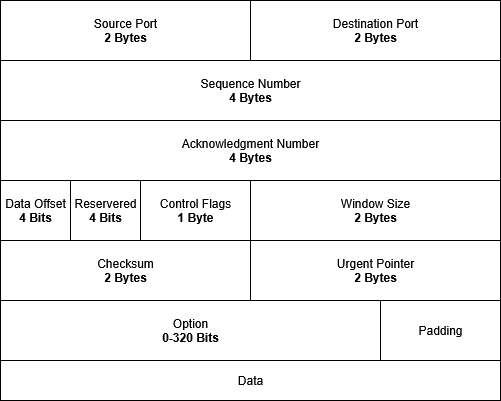
\includegraphics[alt={A block diagram of the TCP header format, detailing its fields and their sizes.}, height=8cm]{./images/tcp_header.png}
	\caption{The TCP header}
	\label{fig:tcp_header}
\end{figure}
The TCP header, figure~\ref{fig:tcp_header}, encodes the functionality of the TCP.
It follows the IP header in a datagram. The header is usually 20 bytes long, but
can be extended using options. It begins with the source and destination port, which
together with the source and destination addresses, are used to identify the connection.
The next two fields in the header are the sequence and acknowledgement numbers. The
sequence number is the sequence number of the first data byte in the data segment.
If the SYN flag is set the sequence number is referring to the initial sequence number
(ISN). The acknowledgement refers to the next sequence number the receiver is
expecting to receive, at the same time acknowledging that all sequence numbers
up to this point was received. Next is the data offset field, indicating where
the data begins. The reserved field following this must be 0. After this is the
1 byte flags field
\begin{itemize}
	\item \textbf{URG} Urgent pointer field is set
	\item \textbf{ACK} acknowledgement field is set
	\item \textbf{PSH} Push function, requesting that buffered data is sent immediately to the receiver
	\item \textbf{RST} Reset the connection
	\item \textbf{SYN} Synchronize sequence numbers
	\item \textbf{FIN} Sender is done sending data
\end{itemize}
The 2 byte window field specifies the number of bytes that may be in-flight at any one
time. This is the specified size of the sliding window that is used for flow
control purposes. Following the window field is a 2 byte checksum field, used for
detecting corruption of the TCP-header, data payload as well as a pseudo IP header,
containing information about the source and destination addresses, as well as the
protocol number and tcp packet length. In case the URG bit is set in the flags field,
the 2 byte urgent pointer header field indicates where the urgent data ends. Finally
the options field contains extension to the normal TCP header, containing among other, options
for maximum segment size and multipath TCP\cite{rfc8684}.

To ensure reliable delivery of TCP segments, each segment is assigned a sequence number.
This allows the receiver to reconstruct segments delivered out of order, and additionally
detect missing segments. The receiver sends acknowledgments, containing the next
expected sequence number, to signal to the sender that the data was successfully received.
The sequence number is a 32 bit number, with the initial sequence number (ISN)
selected randomly at the time when the TCP connection is established. This ensures that
sequence numbers from stale connections have a low probability of overlapping with
any active connection\cite{rfc793}.

The TCP connection is established via a three-way handshake. The client sends
a TCP packet with the SYN bit set in the flags field, this packet contains the
clients ISN. The server responds with a packet with the SYN and ACK bit set,
acknowledging the clients sequence number as well as providing the servers ISN.
Finally the client responds with an ACK, acknowledging the servers ISN. Following
this the client and server are synchronized, and communication may begin. A peer
may terminate its side of the connection by sending a FIN packet, signaling to
the other endpoint that one side has closed its side of the communication. The
closed endpoint may continue receiving data until the other endpoint also closes
it side\cite{rfc793}.
\subsubsection{User Datagram Protocol}
\begin{figure}[b]
	\centering
	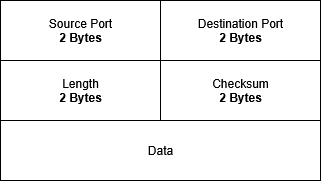
\includegraphics[alt={A block diagram of the UDP header format, detailing its fields and their sizes.}, height=4cm]{./images/udp_header.png}
	\caption{The UDP header}
	\label{fig:udp_header}
\end{figure}
The UDP, which was defined by RFC 768, is designed to
enable programs to transmit self-contained messages, know as datagrams, over a
packet-switched network. The UDP is designed to run on top of the IP\cite{rfc791},
using IP addresses and port numbers for addressing. The UDP is by design connectionless,
providing no guarantees for datagram delivery, duplicate datagrams or in-order
delivery. In exchange, the UDP aims to minimize the overhead present in the protocol.
As UDP is connectionless there is no need to establish a connection via a handshake,
instead datagrams can be transmitted directly, and they should be designed in
such a way that they can stand on their own. The UDP header, as seen in figure~\ref{fig:udp_header}
is only 8 bytes long,
consisting of the source and destination port, as well as the length of the datagram
and a checksum to verify the received datagram\cite{rfc768}. Even though UDP has
a checksum field its use varies depending on the implementation. Some implementations
may discard the datagram, or alternatively pass it along to the application with a 
warning, as UDP provides no way to recover from broken datagrams\cite{computer_networking}. The minimal UDP
header (8 bytes) combined with the lack of a handshake makes UDP a protocol with
the bare minimum needed for datagram transfer.
Generally, UDP is used for applications where low latency is a requirement and some
amount of packet loss is deemed acceptable. It is then up to the application layer to
handle missing, reordered or duplicate datagrams.
\subsection{The Server Message Block protocol}

\clearpage

\section{QUIC}
The Internet's underlying infrastructure is in a state of constant evolution,
driven by a demand for decreased latency, increased throughput requirements and
a need for improved security. For many years now, the TCP has been the de-facto
solution for reliable and secure, when combined with Transport Layer Security (TLS), communications. However,
TCP was developed in a time where security and latency where not considerations,
at least not in the same way as in todays landscape. Over the years there have
been efforts to enhance TCP, such as multipath TCP\cite{rfc8684} and combining
TCP and TLS in HTTPS\cite{rfc2818} to improve security. This section of the thesis
will cover QUIC, a transport protocol developed to overcome the limitations and
improve the performance as compared to the TCP\cite{quic_transport_protocol_design}.

The importance of the QUIC protocol is not to be underestimated. It represents
a substantial change to the internet's transport layer, the first one in over
two decades. QUIC was initially developed by Google, and then later standardized
in RFC 9000\cite{rfc9000}. QUIC is designed to address the issues experienced
by TCP, with a focus on optimizing for web traffic. The main issues being the
Head-of-line (HOL) blocking, but also aiming to improve on other aspects,
such as integrating the TLS handshake into the transport handshake. A decision
that was made for QUIC specifically was to move the protocol out of the kernel
space and into the user space, allowing for rapid development and innovation\cite{quic_transport_protocol_design}.

This chapter of the thesis will outline the limitations of TCP that led to the
development of QUIC, give an overview of the architecture and logic that drives
QUIC.
\subsection{The motivation for a new transport protocol}
The TCP is a cornerstone of modern internet infrastructure. It has been a reliable
work horse for more than 40 years, ensuring communications between users and hosts
since its inception. However, as the design of TCP is largely colored by the
landscape when it was created, much of the improvements that have been made to TCP,
such as security, has had to be built on top of TCP, as these were not considerations
at the time of the TCP's inception. Todays internet landscape, with real-time content,
hyper mobile users and increased demands on latency, but also privacy and security, have exposed
some of the limitation imposed by the TCP stack. This section will outlined the
key issues that prompted the development of a new, modern protocol: QUIC.

\subsubsection{Head-of-Line Blocking}
The TCP guarantees that all frames will be delivered, reliably in-order. Seeing
as the TCP works as a single byte-stream the creates a phenomenon know as
Head-of-Line (HOL) blocking, where any lost packet will block the delivery of
all subsequent packets until the missing packet has been retransmitted. This
can potentially amplify issues in the network, increasing delays, decreasing
throughput and worsening the user experience. To combat this limitation, modern
network protocols, such as HTTP/2\cite{rfc9113}, have introduced measures to
combat the issue. HTTP/2 introduced multiplexing of multiple requests over one
connection, allowing multiple application-level streams, for example for different
resources such as images or javascript, to be multiplexed over a single TCP
connection. This means that HTTP/2 managed to mitigate application-level HOL
blocking, which was an issues in earlier versions of HTTP, it still potentially
suffered from transport level HOL blocking, as the multiplexed streams was still
sent over a single TCP connection. As a result a single lost packet in the TCP
stream still caused all other unrelated streams over the same connection to stall,
even if their packets were successfully delivered, until the offending packet
could be retransmitted. This in practice means that much of the improvements made
by HTTP/2 in this regard was negated by the issues of TCP, particularly in lossy
environments\cite{http2_vs_1}.

\subsubsection{Handshake Delay}
A limitation of the TCP stack is the delay caused by the TCP handshake. As discussed
in earlier chapters, establishing a TCP connection is done via a three-way handshake
(SYN, SYN-ACK, ACK). This handshake incurs one Round-Trip Time (RTT) of delay. In
addition, most application use TLS for security, and historically the TLS 1.2 handshake
and setup adds two additional RTTs of delay. While network bandwidth is ever increasing,
much of the communication done on the internet consist of short dialogues, that
are significantly impacted by the additional overhead brought on by the TCP plus TLS
handshake\cite{quic_transport_protocol_design}.

Some of the latency brought on by the TLS handshake is addressed by TLS 1.3, adding
support for 1-RTT and 0-RTT handshakes, at the cost of perfect forward secrecy\cite{rfc8446}. Even with
these enhancements, the TCP plus TLS handshake takes a minimum of 1,5 RTTs, due to the separation
of connection and security handshake.

\subsubsection{Protocol Ossification}
A big hurdle in deploying new protocols and extensions to existing ones on the internet,
is the protocol ossification of existing protocols on the internet. There exists a heap
of middleboxes, such as Network Address Translators (NATs) and firewalls that are
part of the network. These devices may be overly conservative, dropping or 
modifying packets that do not conform to their assumption. This is already an
issue for TCP enhancements, and entirely new protocols have no chance of reaching
their destination, without explicitly adding support in all necessary middleboxes.
To get around this, protocol designer have to design their protocols from the ground
up to be middlebox proof, such as QUIC encapsulating its protocol inside UDP as an
anti-ossification measure\cite{Ossification}.

A related issue of rolling out enhancements to existing protocols is that the
network stack tends to be part of the Operating System (OS) kernel. The networking
stack is tightly coupled to the OS, requiring OS updates or upgrades to implement
changes to existing protocols. With todays upgrade frequency it can take years
to roll out simple changes to the networking stack. QUIC moves the deployment of the 
protocol to the user space, improving the speed of development and deployment,
and opening up the space for multiple actors to create their own implementations of
the protocol\cite{quic_transport_protocol_design}.

\clearpage

\section{The Server Message Block protocol}

\subsection{Information about the SMB protocol}
\clearpage
\section{Implementing QUIC as transport for SMB server}

\subsection{MsQuic architecture and API}

\subsection{Fusion SMB server QUIC transport layer design}
\clearpage
\section{Performance and interoperability benchmarking}

\subsection{Test environment}

\subsubsection{Hardware environment}

\subsubsection{SMB over QUIC implementations analyzed}

\paragraph{Windows SMB client/server}

\paragraph{Fusion SMB server}

\subsection{Test scenarios}

\subsubsection{interoperability tests}

\subsubsection{Becnhmarking workloads}

\subsection{Results}
\clearpage
\section{Conclusions}
\label{sec:summary}

\subsection{Discussion}

\subsection{Future work}

\clearpage
%% Bibliography/ list of references
%%
%%\nocite{*} % print uncited references in the bibliography
\printbibliography[heading=bibintoc] %, add the title to the table of conten

\end{document}
